\section{团队复制：个人表达如何进入工业化协作}

本章先给结论：个人创作方法要变成团队能力，关键在于把“判断”拆成可协作的结构，同时保留关键创意节点上的经验把关。Tim 的做法保留创作把关；他仍至少会过稿，用上一章的快乐、知识、共鸣、节奏四个要素反复拷问选题和脚本，同时让团队成员拥有自由发挥的空间。\footnote{源时间：00:40:37--00:41:27。} 这给内容公司一个现实答案：可复制的是角色、接口、复盘和资源配置；需要持续训练的是创作者对观众、题材和节奏的判断。

刘润在这一处把问题从“Tim 个人怎样做爆款”推进到“团队怎样复制方法”。如图~\ref{fig:method-to-team} 所示，访谈字幕直接提出“把这个方法”复制到团队里。

\begin{figure}[htbp]
  \centering
  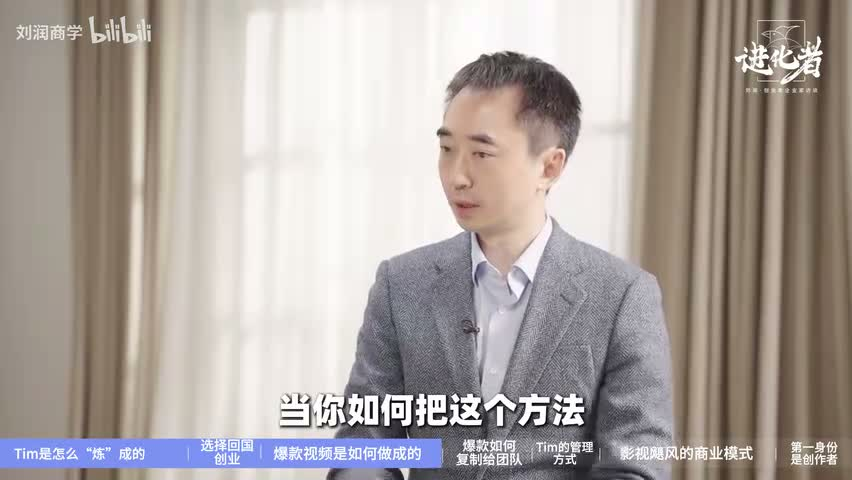
\includegraphics[width=0.70\linewidth,height=0.30\textheight,keepaspectratio]{figures/selected/frame_00-40-38_method_to_team.jpg}
  \caption{从个人方法论转向团队复制：问题的焦点从爆款模型进入组织能力。\protect\footnotemark}
  \label{fig:method-to-team}
\end{figure}
\footnotetext{视频画面时间区间：00:40:37--00:40:44。}

\subsection{复制的边界：Tim 仍然过稿}

团队复制的第一条边界，是最高价值的视频仍要有人承担终局判断。Tim 的回答很清楚：他至少会过稿，未必亲自深度参与每一个制作环节；同时，他也意识到个人投射过重会让每个人身上都刻上自己的影子，这会偏离他的目标。\footnote{源时间：00:40:48--00:41:05。} 这句话的管理含义很重要：团队需要标准，也需要每个创作者形成自己的判断肌肉。

所谓“过稿”，在这里可以理解成一个创意质量闸口。编导可以提出选题、写脚本、组织素材，制片可以安排预算、周期和外景条件，后期可以完成剪辑与节奏，但超级爆款仍要回到几个底层问题：

\begin{enumerate}
  \item 这条内容能否带来快乐，是否具有分享时的轻松感、兴奋感或幽默感？
  \item 它有没有知识增量，观众看完后能否复述一个新信息或新视角？
  \item 它能否触发共鸣，让观众把自己的经历、愿望或情绪投射进去？
  \item 它的节奏是否能支撑从开场、铺垫、转折到结尾的观看动力？
\end{enumerate}

短视频或常规内容可以把某一个属性拉满；超级爆款通常需要多项同时成立。\footnote{源时间：00:41:07--00:41:27。} 因此，方法复制要让每个岗位在自己的环节里看见这些问题，同时避免把每个人塞进同一套模板。编导看选题和脚本，制片看可执行性和风险，后期看节奏与情绪曲线，Tim 的过稿则负责把分散判断重新校准到作品整体。

\subsection{内容矩阵：专业/大众与长/短视频}

当团队达到 100 多人，内容公司无法只围绕单一账号运转。Tim 介绍，团队总共 100 多人，做内容的人差不多 60 多人，其中编导约 20 位，制片约 10 位，剩余是技术型工种，并统一纳入企划与内容相关部门。\footnote{源时间：00:41:33--00:41:53；00:46:12--00:46:24。} 这组数字说明，影视飓风的生产单元已经从个人频道进入组织型内容工厂。

Tim 用一个二维矩阵组织账号和内容定位：一条轴是专业与大众，另一条轴是长视频与短视频。\footnote{源时间：00:41:57--00:43:29。} 这个矩阵的价值在于让团队知道“该做什么”和“用什么成本结构做”。

\begin{table}[htbp]
  \centering
  \caption{内容矩阵：用账号定位约束团队分工}
  \label{tab:content-matrix}
  \begin{tabular}{lll}
    \toprule
    维度 & 代表内容 & 协作含义 \\
    \midrule
    专业长视频 & 影视飓风评测、大型项目、离谱挑战 & 高投入、高技术密度，需要编导、制片、技术协同 \\
    大众长视频 & 一点点不一样、自然科学、人文发现、动物拍摄 & 需要外景、专业顾问、长期题材储备 \\
    大众短视频 & 公司团队 VLOG、氛围与社群内容 & 轻量、高频，强化公司人格和社群连接 \\
    专业短视频 & 短片、短剧与行业热点项目 & 需要明确类型能力和快速试错 \\
    \bottomrule
  \end{tabular}
\end{table}

矩阵背后有一个商业现实：单个频道的广告营收有上限，内容公司需要多个内容产品承接不同受众和不同收入结构。\footnote{源时间：00:42:04--00:42:21。} 这也是组织复制必须面对的资源约束。长视频投入常是短视频的 5--10 倍，尤其是专业长视频和大众长视频，拍摄、交通、设备、安全、专家沟通都会显著抬高成本。\footnote{源时间：00:43:21--00:43:29。}

\subsection{工业化协作：创意需要角色、接口、反馈和约束}

本章的核心概念是“工业化协作”。它指的是把内容生产拆成若干可协作岗位，让创意、脚本、制片、拍摄、技术、后期、发布和复盘形成一条稳定链路。它像高级餐厅从主厨单店扩张到多店经营：口味判断仍然重要，菜单、采购、备料、出餐节奏、成本核算和顾客反馈也必须被拆成明确接口。内容公司同理，创意判断依然在场，协作链路负责把判断放大到更多项目。

从第一性原理看，创意工作的难点来自高度不确定性。观众会不会被打动，天气会不会改变，设备能否承受外景，专家表达能否转化成大众叙事，平台节奏会不会改变，这些都无法在开拍前完全算准。团队化解决的基本问题，就是把一个人的大脑压力分解到多个专业单元：

$$
Q_{\text{team}} \approx h(J, R, I, F, B)
$$

其中：

\begin{itemize}
  \item $Q_{\text{team}}$：团队最终交付的内容质量，是观众体验、制作完成度和传播结果的综合。
  \item $J$：创意判断，包括选题价值、情绪方向、知识密度和节奏感。
  \item $R$：角色分工，包括编导、制片、技术、后期、专家顾问等岗位。
  \item $I$：协作接口，指脚本交付标准、预算边界、拍摄清单、素材命名、过稿节点等连接方式。
  \item $F$：反馈机制，包括成片复盘、数据回看、观众反馈、知识沉淀。
  \item $B$：资源约束，包括预算、周期、体力、安全、商业收入上限和团队人数。
\end{itemize}

这个公式是本章的教学化概括，原视频没有给出数学表达。它的作用是提醒读者：团队复制的瓶颈通常出现在某个变量缺失。只有创意判断，项目会卡在执行；只有岗位分工，作品容易失去灵魂；只有自由环境，结果可能漂移；只有过程控制，创意波动又会被压死。

\begin{figure}[htbp]
  \centering
  
\includegraphics[width=0.86\linewidth,height=0.42\textheight,keepaspectratio]{figures/generated/fig_team_industrial_chain.pdf}
  \caption{团队工业化协作链路：编导、制片、专职人才与复盘共同把个人方法变成组织资产。教学化生成图，综合自 00:27:07--00:28:12 与 00:41:30--00:46:38。}
  \label{fig:team-industrial-chain}
\end{figure}

\begin{importantbox}{团队复制成立的条件}
一个个人创作方法能够进入百人团队，至少要满足五个条件：第一，核心判断有人负责，Tim 仍然在关键稿件上把关；第二，岗位分工足够清楚，编导、制片、技术和专家知道各自承担什么风险；第三，协作接口稳定，脚本、预算、周期、素材、过稿和复盘都有可交接的标准；第四，反馈能沉淀，团队能把一次项目里的教训转成下一次项目的知识；第五，资源约束被公开看见，长视频的高投入、外景风险和商业上限都进入决策。
\end{importantbox}

\subsection{冰岛火山案例：专精化招聘从风险里长出来}

冰岛火山案例说明，工业化协作有具体代价。Tim 讲到团队原本应有更多人去冰岛，因签证问题最后只有少数人前往；他们背着约 30 公斤设备走了约 20 公里山路，到山上拍到火山后，夜里温度从 14 度迅速降到零下 5 度，风很大，衣服不够，团队出现失温风险，其中有人甚至开始出现幻觉。\footnote{源时间：00:43:31--00:45:04。} 这个案例很硬：一条好看的大众长视频，背后可能是设备重量、路线规划、天气窗口、安全预案和体能消耗的复合问题。

从观众视角看，火山节目是“漂亮”“震撼”“稀缺”。从制片视角看，它是预算、签证、设备、路线、保险、天气、人员体能和撤离方案的组合。创意越大，执行风险越高；执行风险越高，岗位专业化越必要。Tim 也因此提到，团队后来意识到只招会拍的人还不够，需要生物背景、户外经验，以及懂具体领域的编导或人才。\footnote{源时间：00:45:07--00:46:12。}

这一点尤其值得内容创业者警惕：当题材从室内评测扩展到自然科学、人文发现和野外项目时，“会拍”只是最低门槛。真正决定作品上限的，是能否把专业知识转成可信叙事，把现场风险转成可执行计划，把专家表达转成观众能理解的发现。Tim 对“一点点不一样”的定位也体现了这种边界意识：他们讲述发现，请行业里真正厉害的专家来讲，避免用创作者自己的嘴去冒充专业判断。\footnote{源时间：00:45:43--00:46:07。}

\subsection{产品团队与公司内创业：让内容公司多一个增长引擎}

内容团队之外，Tim 还提到产品团队有 20 多人，负责电商产品，也在研发 iPhone 配件等自有产品。\footnote{源时间：00:46:24--00:46:32。} 这部分看似偏商业，其实仍属于团队复制问题。原因很现实：如果一家内容公司只依赖频道广告，营收上限会限制内容投入；如果产品线能够跑出来，内容团队就有机会获得更稳定的资源供给。

Tim 把这件事称作一种赌注：未来有没有可能减少对频道广告赚钱的依赖，并用产品收入养活内容团队。他也承认这很难，目前没有先例。\footnote{源时间：00:46:32--00:46:42。} 这种说法很清醒。产品团队、行政支持和孵化小组共同构成“公司内创业”的结构：每个小组都像一个小型实验单元，在公司品牌、流量、供应链和内容理解的基础上寻找新的业务可能。

这里的未知风险同样需要说透。内容团队擅长注意力、叙事和观众信任；产品团队还要面对供应链、库存、售后、毛利、复购和渠道效率。二者共享品牌资产，能力结构却有明显差异。公司内创业的价值在于让团队可以用小单元试错；它的风险在于任何产品失败都会消耗现金、管理注意力和观众信任。

\subsection{Context vs Control：自由环境要用结果负责}

本章最后回到文化。Tim 说，他很重视公司伙伴，认为一些老式企业更重视 Control，也就是控制；而他更看重 Context，也就是实际内容、产出和情境供给。他把焦点放在周期结果上，成员在周期内可能打游戏，创意也会波动；好的环境可以提供，最终结果必须好。\footnote{源时间：00:47:41--00:48:12。}

\begin{knowledgebox}{Context vs Control}
Control 指过程管束，例如打卡、审批、动作监控和固定流程；Context 指让人能做出好结果的上下文，包括目标、信息、资源、审美标准、团队氛围、时间预算和反馈机制。可以用厨房作类比：Control 像主管盯着厨师每一刀怎么切；Context 像提前讲清菜单定位、食材预算、出餐标准、客人反馈和安全边界，然后让厨师对菜品负责。创意团队需要 Context，因为灵感、选题和脚本会波动；管理仍然需要结果，因为作品最终要接受观众、平台和商业目标的检验。
\end{knowledgebox}

这也是工业化协作最容易被误解的地方。把工业化理解成流程捆绑，会压低创意人员的判断空间；把自由理解成目标缺席，团队结果会漂移。Tim 的管理偏好是减少表层规则，追寻内在结果。他在后文还会继续谈到取消打卡、用量化数据观察结果等做法，这些内容会进入下一章的自由化管理与 OKR。\footnote{源时间：00:49:05--00:49:40。}

因此，本章给出的组织逻辑可以压缩成一句话：用 Context 保护创意波动，用角色和接口降低协作成本，用反馈和资源约束校准结果。这样，团队才能在不抹平个人判断的前提下，把 Tim 的方法扩展为公司能力。

\subsection{本章小结}

个人创作方法进入百人团队，需要完成三次转换。第一，方法从个人经验转成可讨论的判断标准，例如快乐、知识、共鸣、节奏。第二，作品从个人执行转成工业化协作链路，编导、制片、技术、专家、后期和复盘各自承担不同风险。第三，公司从单一内容团队转成多引擎组织，内容矩阵、产品团队和公司内创业共同对冲频道广告上限。

本章最重要的提醒是：团队复制的目标是放大判断，避免抹掉判断。Tim 仍然过稿，说明创作经验在关键节点仍有价值；专业化招聘、冰岛火山案例和 Context vs Control，则说明经验必须被角色、接口、反馈和资源约束承接。下一章将继续解释：当自由成为组织文化，OKR 和结果指标怎样防止自由滑向失控。
